%========= info ===================
% Esta es una plantilla para reportes de laboratorio
% Autor: Philip J Fry
% Licencia: Creative Commons
% ================================

\documentclass[12pt]{report} % Declarando clase de documento
%======= pre-ambulo ==========%
\usepackage[utf8]{inputenc}
% \usepackage[backend=biber, style=ieee, sorting=ynt]{biblatex}
\usepackage[backend=biber, style=apa]{biblatex}
\addbibresource{referencias.bib}

%==== Generador de Texto Dummy ======
\usepackage{lipsum}
%===== Definiendo Idioma Español =======
\usepackage[spanish]{babel}
\selectlanguage{spanish}
%===== Control de Margenes ======
\usepackage[a4paper,tmargin=3cm,bmargin=2.5cm,lmargin=3cm, rmargin=2.5cm, bindingoffset=6mm]{geometry}
%======================================================================================================
% ======= librery graphicx=========
\usepackage{graphicx}
% =================================
% ===== librerias matematicas ==========
\usepackage{amsmath, amssymb, amsfonts}
\usepackage{amsthm}
\usepackage{mathrsfs}
%====== Datos Generales =========
\title{Paper                 Conferencia}
\author{Lenin G. Falconi }
\date{Abril, 2020}
%======= Documento ==============
\begin{document}

\maketitle
\tableofcontents
\section{Introducción}
En \cite{nogueira2017image} se       dispone de una revisión sistemática de la literatura. Sin embargo, la propuesta indicada en \cite{dawkins_biology_2016} contradicen lo habitual. El trabajo propuesto por \cite{priandana2018backprop} utiliza el algoritmo de \textit{backpropagation} para controlar un robot de rueda. El niño estudia todas las noches.

\lipsum[2-4] 

\section{Revisión de Literatura}
\subsection{Cadena de búsqueda}
\lipsum[1-4]
\subsection{Criterios de inclusión y Exclusión}
\lipsum[1-4]
\subsection{Extracción de Información}
\subsubsection{Criterios de Calidad}
\lipsum[1-4]
\subsubsection{Amenazas de Validez}
\lipsum[1-4]
\subsection{Discusión}
\citeauthor{dawkins_biology_2016} (\citeyear{dawkins_biology_2016}) afirma que agnosticismo es una filosofía incompleto. \citeauthor{nogueira2017image} (\citeyear{nogueira2017image}) contradice la anterior afirmación y presenta un ejemplo. Finalmente, se ha demostrado que es un filosofía válida \parencite[ver pag 92]{priandana2018backprop}. "El agnosticismo indica que hay un 50\% de verdad en la tesis uno y en la tesis dos" \textcite{nogueira2017image}. La Figura \ref{fig:arquitecturaRedConv} representa una red neuronal convolucional tradicional. \textcite{saha2018} afirma lo siguiente.

\begin{figure}[h!]
    \centering
    % scale, width=\columnwidth
    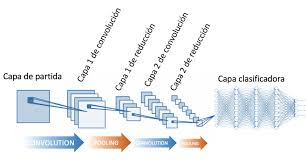
\includegraphics[width=0.7\textwidth]{imagenes/convnet.jpeg}
    \caption{Arquitectura Red Neuronal Convolucional}
    \footnotesize{Imagen tomada de \textcite[Capítulo 1, pág. 23]{nogueira2017image}}
    \label{fig:arquitecturaRedConv}
\end{figure}

\lipsum[3] La Figura \ref{fig:autoencoder_Estructura} muestra algo intersante \parencite{alberti2018} 23.5\% esto no aparecera en el pddf.

% Insertar figura 
\begin{figure}[h!]
    \centering
    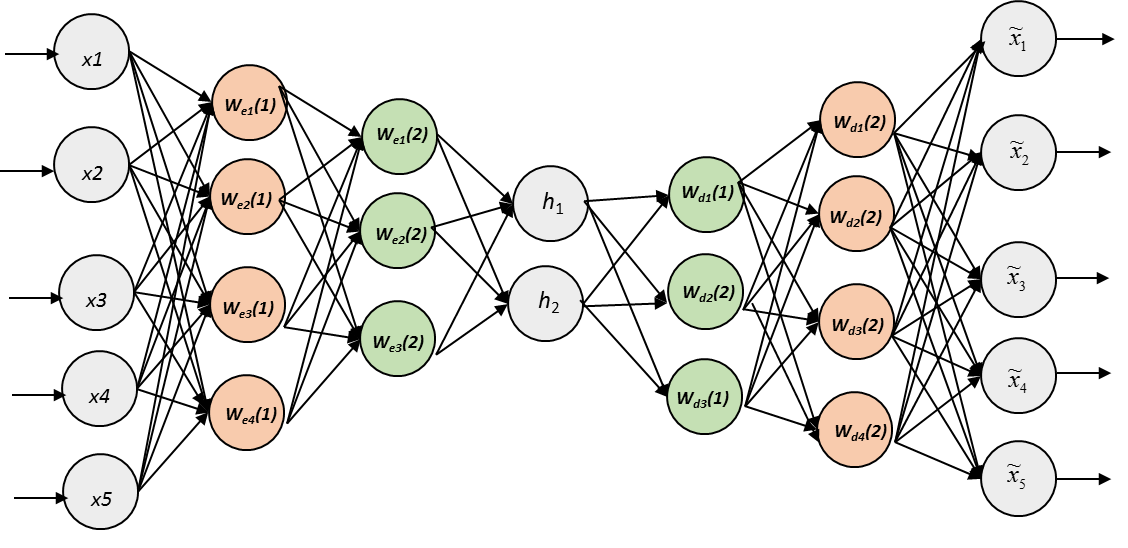
\includegraphics[width=\textwidth]{imagenes/autoencoder.png}
    \caption{Estructura de un Autoencoder}
    \label{fig:autoencoder_Estructura}
\end{figure}

\section{Metodología}
\lipsum[1-4]
\newpage
\section{Resultados Experimentales}
Aqui voy a poner los resultados tabulados de mi experimento. En la Tabla \ref{tab:mis_mediciones} se presentan las mediciones realizadas en el experimento indicado en la Sección.

\begin{table}[htbp]
    \centering
    \caption{Medidas Experimentales}
    \begin{tabular}{|ccc|}
        \hline
        \textbf{Presion} & \textbf{Temp} & \textbf{Vol}  \\ \hline
         2.30   &  24.5 & 34.5 \\
         7.30   &  64.5 & 24.5 \\
         8.30   &  14.5 & 24.5 \\ \hline
    \end{tabular}
    \label{tab:mis_mediciones}
\end{table}{}

La Tabla \ref{tab:mis_otras_mediciones} muestra un comportamiento interestante.

\begin{table}[h!]
\centering
\caption{Otras Medidas}
\begin{tabular}{ll|ll}
\multicolumn{2}{c|}{\textbf{Var1}} & \multicolumn{2}{c}{\textbf{Var2}} \\ \hline
\textbf{a1}          & 12          & 12              & 45              \\
\textbf{a2}          & 34          & 65              & 78             
\end{tabular}
\label{tab:mis_otras_mediciones}
\end{table}

En la Tabla \ref{tab:comparacion} se comparan los resultados de los diferentes autores. 

% Autor, Titulo, Resultado
\begin{table}[h!]
\centering
\caption{Comparacion de Resultados}
\begin{tabular}{ccc}
\textbf{Autor}    & \textbf{Año}    & \textbf{Resultado} \\ \hline
    \citeauthor{priandana2018backprop} &    \citeyear{priandana2018backprop} & 0.9                \\
    \citeauthor{dawkins_biology_2016}  &    \citeyear{dawkins_biology_2016}  & 0.8                \\
    \citeauthor{nogueira2017image}     &    \citeyear{nogueira2017image}     & 0.7                \\ \hline
\multicolumn{2}{c}{\textbf{Promedio:}} & 0.8               
\end{tabular}
\label{tab:comparacion}
\end{table}

La teoria de la relatividad afirma $E = mc^{2}$. Mientras que el producto esecalar entre los vectores $\vec{v_{1}}$ y $\vec{v_{2}}$ es 0. La Ecuacion \eqref{eq:ecuacion1} que relaciona el espacio vectorial $\mathcal{X}$ con $\mathcal{Y}$ es, $x \in \mathbb{R}^{3}$:

\begin{equation}
    \label{eq:ecuacion1}
    \hat{y}_{\theta} = ax^{2}
\end{equation}

\section{Conclusiones y Trabajos Futuros}
\begin{itemize}
    \item suceso1
    \item suceso 2
    \item suceso 3
\end{itemize}

\begin{enumerate}
    \item suceso1
    \item suceso2
    \item suceso3
\end{enumerate}

\printbibliography[title={Bibliografía}]

\end{document}
